\documentclass[12pt]{article}
\usepackage{verbatim}
\usepackage[dvips]{epsfig}
\usepackage{color}
\usepackage{url}
\usepackage[colorlinks=true]{hyperref}

\begin{document}

\section*{GENESIS: Documentation}

{\bf Related Documentation:}
% start: userdocs-tag-replace-items related-do-nothing
% end: userdocs-tag-replace-items related-do-nothing

\section*{g-tube Technical Specification}

	This document outlines the design process employed in the development of the {\bf g-tube}, a graphical user interface which brings all components of the {\bf GENESIS3} system together. With the {\bf g-tube} a user can load, create and run models, track all aspects of the simulation including the schedule, parameters, models, underlying software versions, and directly load the output of simulation runs into {\bf Atoms} that can be processed into tables, plots, and formatted text suitable for inserting into manuscripts. The end result of a {\bf g-tube project} will be a compiled electronic publication, containing the finalized document, with all of the data used to generate the figures {\bf tag-associated}  with the model experiment runs. 

\section*{History}

	

\section*{Data Design}

\subsection*{Project Specification}

	A project is a class data structure that is used to track all work done by the user within the {\bf g-tube}. Projects are treated as a combination of categorized lists of data that grow and shrink as the user goes through the {\bf user workflow}. Data tracked includes:
	
\begin{itemize}
	\item[] Project name.
	\item[] List of atoms.
	\item[] Manuscript pages.
	\item[] GUI perspective state.
\end{itemize}

From a file storage perspective a project consists of a directory containing all files in the users workspace along with a {\bf yaml} file that bears the same name as the project. The {\bf yaml} file provides a mapping for all of the files in the project directory so that they can be loaded by the appropriate data management objects within the GUI.

\subsection*{Object Relationships}

	The {\bf g-tube} is set up with a set of "management" classes; their purpose is to provide high level control for the GUI to work with all of the underlying systems, without allowing code from unrelated systems to interlace with one another. This separation allows these complex data management classes to be developed and tested separately.

\begin{itemize}
	\item[] {\bf Project Manager:} Loads or creates a project specification and allows for creating, deleting and editing Model, Atom, Manuscript, and Review management objects.
	\item[] {\bf G3 User Workflow Manager:} Manages a list of models associated with the current project, along with model states and {\bf SSP} configurations.
	\item[] {\bf Atom Manager:} Manages a list of all of the atoms in the current project. 
	\item[] {\bf Manuscript Manager:} Manages the atoms tagged as part of a manuscript.
	\item[] {\bf Review Manager:} Manages the compiled manuscript atoms for review.
\end{itemize}

\begin{figure}[ht]
   \centering
   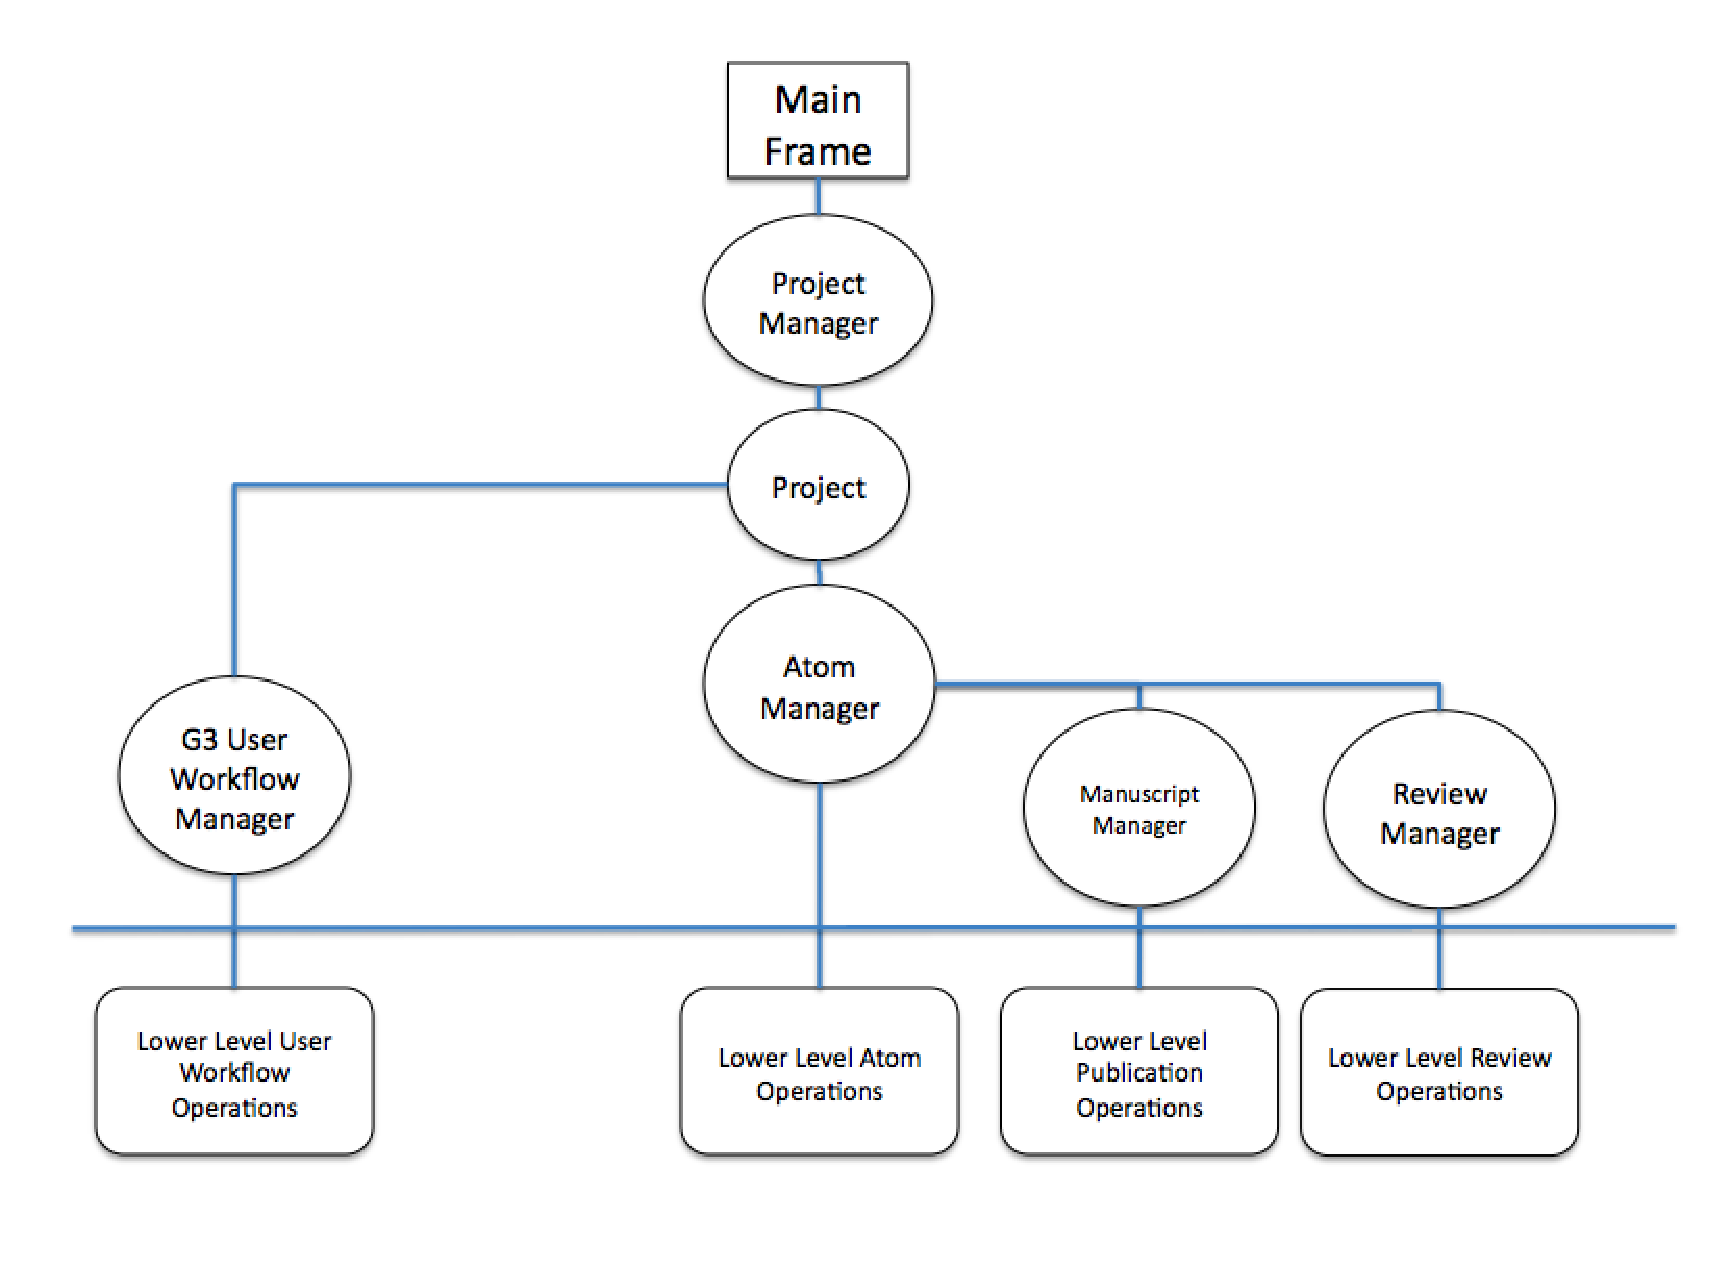
\includegraphics[scale=0.50]{figures/Overview.eps}
   \caption{{\bf Object overview:} A general overview of class relationships within the g-tube.}
   \label{figure: 1}
\end{figure}

The Atom management object allows for basic list operations such as adding, deleting, and editing members. Manuscript and Review managers are subclasses of the Atom manager, that display tag-filtered views of atoms in the project workspace. Management objects encapsulate {\bf wxPython} operations for allowing the end user to perform these actions graphically by drawing their control widgets to the Main Frame. 

\subsection*{Model Object}

	To constrain the complexities of interfacing with the whole of the {\bf GENESIS3} system, modeling functionality is isolated to a single class. In principle this should allow other simulators to be encapsulated within the same abstract data type so long it is mapped to the predefined inputs and outputs the {\bf ModelManager} uses to communicate with the rest of the system.
	Currently interfacing is done via the {\bf gshell} over file descriptors via the object class called {\it bridge}. 
	
\subsection*{Project Explorer Tabs}

	To navigate the various files the user works with in a project there are four tabs which correspond to each management class. Each tab functionality is categorized as such:
	
\begin{itemize}
\item[] G3 User Workflow
\item[] Content Selection
\item[] Model Validation
\item[] Review Validation
\end{itemize}


\section*{Architecture Design}

Working on this.


\section*{Interface Design}

\subsection*{UI Real Estate}

Presentation of widgets is implemented with the {\bf wxPython} Advanced User Interface (AUI) toolkit. This allows for several dockable panes that the user can rearrange to their liking. 

\begin{figure}[ht]
   \centering
   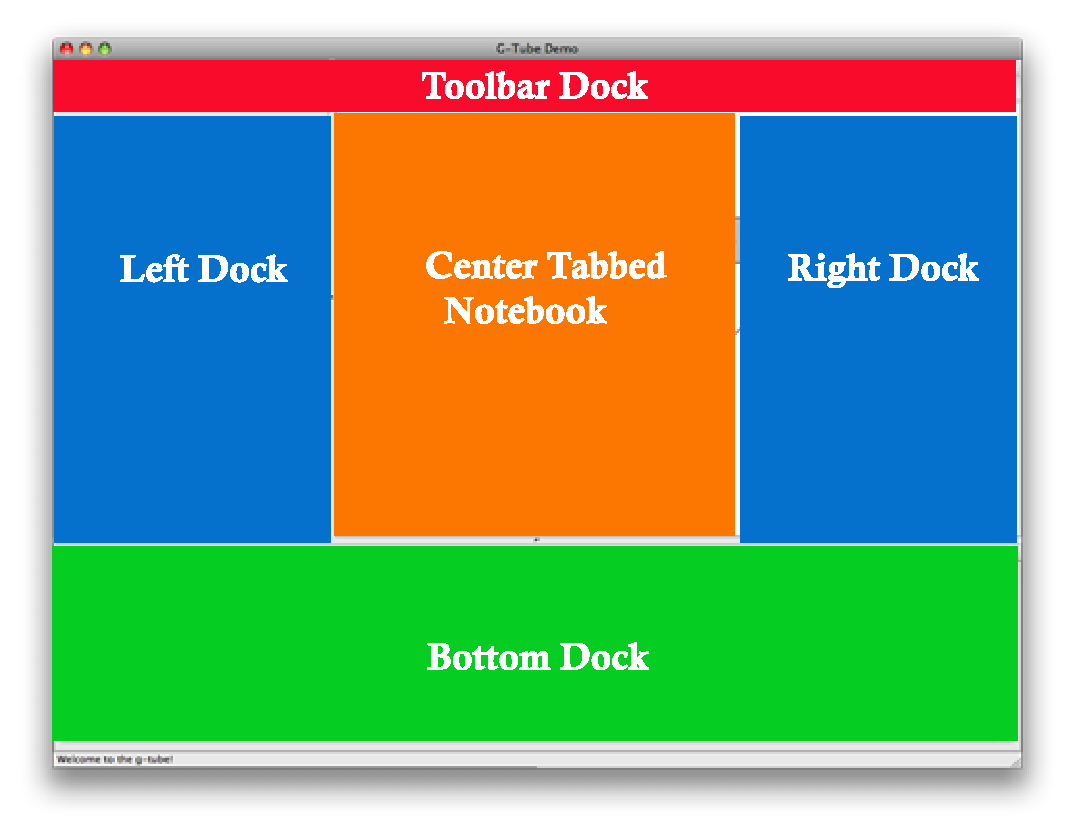
\includegraphics[scale=0.6]{figures/RealEstate.eps}
   \caption{{\bf Main Frame Layout:} Figure shows the default layout of the frames dockable panels.}
   \label{fig:Real Estate}
\end{figure}

\begin{itemize}
\item[] {\bf Toolbar Dock:} Holds icon labeled buttons for performing many shortcuts within the system. Toolbars can be removed from the dock and allows to float at different areas of the screen.
\item[] {\bf Left Dock:} The primary dock for explorer widgets used to manage data in the {\bf Model}, {\bf Atom}, {\bf Manuscript}, and {\bf Review} workspaces.
\item[] {\bf Center Tabbed Notebook:} The "main" workspace. All data selected from a workspace via an explorer will be displayed in a Tab in the Center Notebook. E.G Editable Documents, Manuscript Atoms, Plots from simulation.
\item[] {\bf Right Dock:} Primarily used to hold widgets for editing attributes (such as tags) to the current working tab in the Center Notebook.
\item[] {\bf Bottom Dock:} Primarily holds widgets that output data from the underlying system. E.G Console output from the {\bf g-tube}, model status, error messages.
\end{itemize}

\section*{Procedural Design}

\subsection*{Development Tools}

	The implementation of the {\bf g-tube} is done in {\bf Python} using the {\bf wxPython} widget toolkit. The {\bf wxPython} toolkit is a Python extension module of the popular {wxWidgets} coss-platform GUI library. This allows the user to create widgets with the look and feel of the host operating system while using the powerful {\bf Python} language. {\bf wxPython} is open source, has many contributors, boasts a large collection of example tutorials and documentation, and possesses one of the friendliest communities.
	
Other external Python modules used include:

\begin{itemize}	
\item[] {\bf yaml:} For parsing and loading configuration and data files.
\item[] {\bf matplotlib:} Provides more refined plot panels.
\end{itemize}

Higher level GUI construction is done using \href{http://xrced.sourceforge.net/}{\bf XRCed}, a simple graphical editor that creates Python classes with embedded (or externally loaded) \href{http://wiki.wxpython.org/XRCTutorial}{\bf XRC} files. 

\subsubsection*{Engineering Tools}

For UML and other software figure drawing a "project" directory has been placed in the top level source code directory. In this directory there is are project files for:

\begin{itemize}
\item[] \href{http://bouml.free.fr}{\bf bouml}: A freeware cross platform UML diagramming software. It features a wealth of user \href{http://bouml.free.fr/doc/index.html}{documentation} and can export Python code from your diagrams.
\item[] \href{http://www.stack.nl/~dimitri/doxygen/}{\bf Doxygen}: Doxygen has a UML option that creates very nice looking diagrams with browsable code.
\end{itemize}

As the project increases in scope and size, engineering tools such as this help to keep the project manageable, especially for programmers wishing to modify existing code.




\end{document}
